
\begin{figure}[htbp]
    \centering
    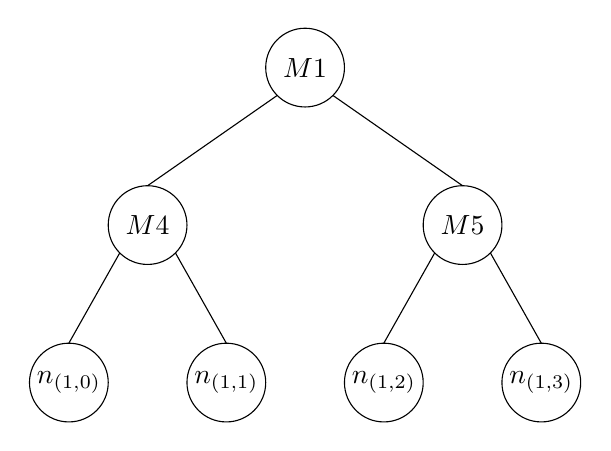
\begin{tikzpicture}[scale=0.5] % Adjust the scale factor as needed
        % Your TikZ code goes here
        \draw (0,0) circle (1cm);
        \node at (0,0) {$M1$};
        \draw (-4,-4) circle (1cm);
        \node at (-4,-4) {$M4$};
        \draw (4,-4) circle (1cm);
        \node at (4,-4) {$M5$};
        \draw (-6,-8) circle (1cm);
        \node at (-6,-8) {$n_{(1,0)}$};
        \draw (-2,-8) circle (1cm);
        \node at (-2,-8) {$n_{(1,1)}$};
        \draw (6,-8) circle (1cm);
        \node at (6,-8) {$n_{(1,3)}$};
        \draw (2,-8) circle (1cm);
        \node at (2,-8) {$n_{(1,2)}$};
        \draw ({0 + cos(225)},{0 + sin(225)}) -- (-4,-3);
        \draw ({0 + cos(315)},{0 + sin(315)}) -- (4,-3);
        \draw ({-4 + cos(225)},{-4 + sin(225)}) -- (-6,-7);
        \draw ({-4 + cos(315)},{-4 + sin(315)}) -- (-2,-7);
        \draw ({4 + cos(225)},{-4 + sin(225)}) -- (2,-7);
        \draw ({4 + cos(315)},{-4 + sin(315)}) -- (6,-7);
        


    \end{tikzpicture}
    \caption{Ways of Merging}
    \label{fig:ways_of_merging}
\end{figure}
